\documentclass[lang=cn,10pt,thmcnt=section]{elegantbook}
\usepackage{graphicx}
\usepackage{float}
\usepackage{esint}
\usepackage{mathtools}
\usepackage{tikz}
\title{数学分析}



\author{Huang}
\date{\today}




\setcounter{tocdepth}{3}


\cover{cover.jpg}

% 本文档命令
\usepackage{array}
\newcommand{\ccr}[1]{\makecell{{\color{#1}\rule{1cm}{1cm}}}}

% 修改标题页的橙色带
% \definecolor{customcolor}{RGB}{32,178,170}
% \colorlet{coverlinecolor}{customcolor}

\begin{document}
	
	\maketitle
	\frontmatter
	
	\tableofcontents
	
	\mainmatter
	\chapter{数列}
	\section{极限的计算}
	\subsection{stolz定理}
	\begin{theorem}[stolz]
		\begin{itemize}
			\item $(\frac{0}{0})$型,$\{ a_n\} ,\{ b_n\}$是无穷小量,$\{ a_n\}$单调递减,$\lim_{n \to \infty}  \frac{b_{n+1}-b_n}{a_{n+1}-a_n}=l$,	则$\lim_{n \to \infty}  \frac{b_n}{a_n}=l$
			\item $(\frac{*}{\infty})$型,$\{ a_n\} $是严格单调递增无穷大量,$\lim_{n \to \infty}  \frac{b_{n+1}-b_n}{a_{n+1}-a_n}=l$,则$\lim_{n \to \infty}  
			\frac{b_n}{a_n}=l$
		\end{itemize}
	\end{theorem}

	\begin{example}
		设 $a_1 \in (0,1), a_{n+1} = \sin a_n, n = 1,2,\cdots$,试计算  
\[ \lim_{n \to \infty} \sqrt[n]{n a_n}. \]
	\end{example}
	\begin{example}
		设 $a_n > 0$ 且  
\[ \lim_{n \to \infty} \frac{a_{n+1}}{a_n} \]  
存在或者为确定符号的 $\infty$。

(1) 求证:  
\[ \lim_{n \to \infty} \sqrt[n]{a_n} = \lim_{n \to \infty} \frac{a_{n+1}}{a_n}. \]

(2) 进一步,若  
\[ \lim_{n \to \infty} a_n = a, \]  
计算  
\[ \lim_{n \to \infty} \left( \frac{\sqrt[n]{a_1} + \sqrt[n]{a_2} + \cdots + \sqrt[n]{a_n}}{n} \right)^n. \]  
(2023中科院夏令营)
	\end{example}
\begin{example}
	\begin{itemize}
		\item 设  
		\[ S_n = \sum_{k=0}^n \frac{\ln C_n^k}{n^2}, \]  
		求  
		\[ \lim_{n \to \infty} S_n. \]
		
		\item 计算  
		\[ \lim_{n \to \infty} \frac{\ln n}{\sum_{k=1}^n \frac{1}{k} - \ln n}. \]  
		(第十二届全国大学生数学竞赛)
	\end{itemize}
\end{example}

\subsection{abel变换}
\begin{theorem}
	\[
\sum_{k=1}^n a_k b_k = \sum_{k=1}^{n-1} (a_k - a_{k+1}) B_k + a_n B_n, \quad \text{其中 } B_k = \sum_{i=1}^k b_i.
\]
\end{theorem}
\begin{example}
	设 $\lim_{n \to \infty} \sum_{k=1}^n a_k$ 存在,试计算 $\lim_{n \to \infty} \frac{1}{n} \sum_{k=1}^n k a_k$.
\end{example}
\begin{example}
	(2023 中科大考研压轴) 设有实数列 $\{a_n\}$, 令 $S_n = \sum\limits_{k=1}^n a_k$, $\sigma_n = \frac{1}{n}\sum\limits_{k=1}^n S_k$。

(1) 证明:若 $\{S_n\}$ 有极限 $S$, 则 $\lim\limits_{n \to \infty} \sigma_n = S$。

(2) 若 $\{\sigma_n\}$ 收敛, 且 $a_n = o\left(\frac{1}{n}\right)$, 则 $\{S_n\}$ 收敛。

\end{example}
\begin{example}
	(2023 中科院提前批) 设 $\lim\limits_{n \to \infty} a_n = a$, $\lim\limits_{n \to \infty} b_n = b$, 试求:

\[
\lim_{n \to \infty} \frac{a_1 b_n + a_2 b_{n-1} + \cdots + a_n b_1}{n}
\]


\end{example}
\subsection{拟合法}
拟合法主要是一种思想,在于抓住问题的关键部分
\begin{example}
	(2023 北师大夏令营) 设 $f \in C[0,1]$,求证:
\[
\lim_{h \to 0^+} \int_0^1 \frac{h}{h^2 + x^2} f(x) dx = \frac{\pi}{2} f(0).
\]

\end{example}
\begin{example}
	(2022 浙大直博压轴) 设 $f(x) \in R[0,1]$,求证:
\[
\lim_{n \to \infty} \int_0^1 f(x) |\sin nx| dx = \frac{2}{\pi} \int_0^1 f(x) dx.
\]

\end{example}
\begin{example}
	\begin{itemize}
		\item 求证:
		\[
		\lim_{n \to \infty} \int_0^{\frac{\pi}{2}} \sin^n x \, dx = 0.
		\]
		
		\item (2022 吉大夏令营改编) 设 $f \in R[0,1]$,且 $f(x)$ 在 $x=1$ 处连续,求证:
		\[
		\lim_{n \to \infty} n \int_0^1 f(x) x^n \, dx = f(1).
		\]
	\end{itemize}
\end{example}
\section{渐进展开}
\subsection{初等方法}
反复利用Stolz定理即可
\begin{example}
	(2021 电子科大考研) 设 $x_{n+1} = \ln(1+x_n)$, $n=1,2,\cdots$, $x_1>0$。试求 
\[
\lim_{n\to\infty}\frac{n(nx_n-2)}{\ln n}。
\]

\end{example}
\begin{example}
	设 $x_{n+1}=\sin x_n$, $n=1,2,\cdots$, $x_1\in (0,\pi)$。计算
\[
\lim_{n\to\infty}\frac{n}{\ln n}\left(1-\sqrt{\frac{n}{3}}x_n\right)。
\]
\end{example}
\begin{example}
	(2023 南大夏令营) 已知方程 $x^n - 2023x = 2023$ 在 $(0,+\infty)$ 上有唯一解 $x_n$,试求极限
\[
\lim_{n\to\infty}\frac{nx_n^n}{\ln n}。
\]
\end{example}
\begin{example}
	\begin{enumerate}
		\item (2020 电子科大考研) 设 $0 < a_n < 1$, $a_{n+1} = a_n (1 - a_n)$,求证:
		\[
		\lim_{n \to \infty} \frac{n a_n}{\ln n} = 1.
		\]
		
		\item (2024 浙大考研) 设 $x_1 = 1$, $x_{n+1} = \sqrt{\frac{2x_n^2}{2 + x_n^2}}$, $n = 1, 2, \cdots$。求证:
		\[
		\lim_{n \to \infty} \frac{n(x_n - x_{n+1})}{\ln (1 + x_n)} = 1.
		\]
	\end{enumerate}
\end{example}
\subsection{迭代方法}
\begin{example}
	设 $x_n > 0$ 且满足 $x_n e^{x_n} = n$, $n = 1, 2, \cdots$,求证:
\[
x_n = \ln n - \ln \ln n + \frac{\ln \ln n}{\ln n} + o\left(\frac{\ln \ln n}{\ln n}\right), \quad n \to \infty.
\]
\end{example}
\begin{example}
	(2024 上交考研) 设 $f \in C(0, +\infty)$,且满足 $x = f(x)5^{f(x)}$,求证:
\begin{enumerate}
    \item $f(x)$ 严格单调递增,
    \item $\lim\limits_{x \to +\infty} f(x) = +\infty$,
    \item $\lim\limits_{x \to +\infty} \frac{f(x)}{\ln x} = \frac{1}{\ln 5}$。
\end{enumerate}
\end{example}
\begin{example}
	(2021 北师夏令营压轴) 给定方程 $x^n(x-1) = 1$,求证:

\begin{enumerate}
    \item 上述方程在 $[1, +\infty)$ 上有唯一根 $x_n$。
    \item 成立不等式:
    \[
    x_{n+1} > 1 + \frac{\ln n}{n} - \frac{\ln \ln n}{n}
    \]
\end{enumerate}
\end{example}
\subsection{Laplace方法}
大体上,Laplace 方法适用于 $\int_{a}^{b} f^n(x)g(x)dx$ 型积分的渐近估计。可以通过变形和换元法转化为标准形式。这种方法的整体思想就是抓极值部分和所谓的局部化原理。
\begin{example}
	(Wallis 公式) 求证:
\[
\frac{(2n)!!}{(2n-1)!!} \sim \sqrt{\pi n}, \quad n \to \infty.
\]
\end{example}
\begin{example}
	(Stirling 公式) 求证:
\[
n! \sim \sqrt{2\pi n}\left(\frac{n}{e}\right)^n, \quad n \to \infty.
\]

\end{example}
\begin{example}
	\begin{itemize}
		\item (2023 吉大夏令营) 已知函数 $f(x)$ 一阶导存在且 $f(1) = 0$,求极限
		\[
		\lim_{n \to \infty} n \int_{0}^{1} x^{n} f(x) \, dx.
		\]
	\end{itemize}
\end{example}

\section{递推数列的敛散性判断}
\subsection{单调性分析方法}
单调性分析方法仅仅适用于
\[
x_{n+1} = f(x_n), \quad n \in \mathbb{N}.
\]
$f$ 是单调递增或是单调递减的情形。

\subsubsection*{结论 1}
设 $f$ 是单调递增函数,则上述递推式确定的 $x_n$ 一定单调,且和不动点的大小关系固定。



\subsubsection*{结论 2}
设 $f$ 是单调递减函数,则上述递推式确定的 $x_n$ 一定不单调,且和不动点的大小关系交错。

\begin{example}
	设 $x_1 > -1$, $x_{n+1} = \frac{1}{1+x_n}$, $n = 1, 2, \cdots$,求极限
\[
\lim_{n \to \infty} x_n.
\]
\end{example}
\begin{example}
	(第十五届全国大学生数学竞赛赛制)设 $x_1 = a = \sqrt[3]{3}$, $x_{n+1} = a^{x_n}$, $n = 1, 2, 3, \ldots$,求证:
\[
\lim_{n \to \infty} x_n
\]
存在但不等于3。
\end{example}
\begin{example}
	\begin{itemize}
		\item 设 $x_1 > -6$, $x_{n+1} = \sqrt{6 + x_n}$, $n = 1, 2, \ldots$, 计算 $\lim\limits_{n \to \infty} x_n$.
		
		\item 设 $x_1 = 2$, $x_n + (x_n - 4)x_{n-1} = 3$, $n = 2, 3, \ldots$, 计算 $\lim\limits_{n \to \infty} x_n$.
	\end{itemize}
\end{example}
\subsection{压缩映像方法}
压缩映像方法是一种非常重要的处理模型。其思想内核有两种。
一种是找到不动点 \( x_0 \),然后得到某个 \( L \in (0,1) \)。s.t.

\[|x_n - x_0| \leq L |x_{n-1} - x_0| \leq \cdots \leq L^{n-1} |x_1 - x_0|\]

另一种是得到某个 \( L \in (0,1) \)。s.t.

\[|x_n - x_{n-1}| \leq L |x_{n-1} - x_{n-2}| \leq \cdots \leq L^{n-2} |x_2 - x_1|\]

当数列的递推式 \( x_{n+1} = f(x_n) \) 确定时,我们有:

\[|x_n - x_0| = |f(x_{n-1}) - f(x)|, \quad |x_n - x_{n-1}| = |f(x_{n-1}) - f(x_{n-2})|\]

因此往往可以通过中值定理或直接放缩来得到 \( L \in (0,1) \)。


\begin{example}
	(2023 中科院提前批)对于给定实数 \( x \),不断将余弦函数作用在之前的数上,得到的序列 \(\{a_n\}\) 如下:\( a_0 = x, a_1 = \cos(x), a_2 = \cos(\cos(x)) \),\(\cdots\),试问当 \( n \to \infty \) 时,这一序列会有怎样的趋势?
\end{example}
\begin{example}
	给定方程 \(x^n + 2023x = 2023\),求证:方程在 \((0,+\infty)\) 只有唯一解 \(x_n\)。且 \(\lim\limits_{n \to \infty} x_n = 1\)。

\end{example}
\begin{example}
	设 \(x_1 > -1, x_{n+1} = \frac{1}{1+x_n}, n = 1, 2, \cdots\),求极限 \(\lim\limits_{n \to \infty} x_n\)。
\end{example}
\begin{example}
	求数列 \(\sqrt{7}, \sqrt{7-\sqrt{7}}, \sqrt{7-\sqrt{7}+\sqrt{7}}, \ldots\) 的极限。
\end{example}
\subsection{蛛网工作法}
\begin{figure}[h]
	\centering
	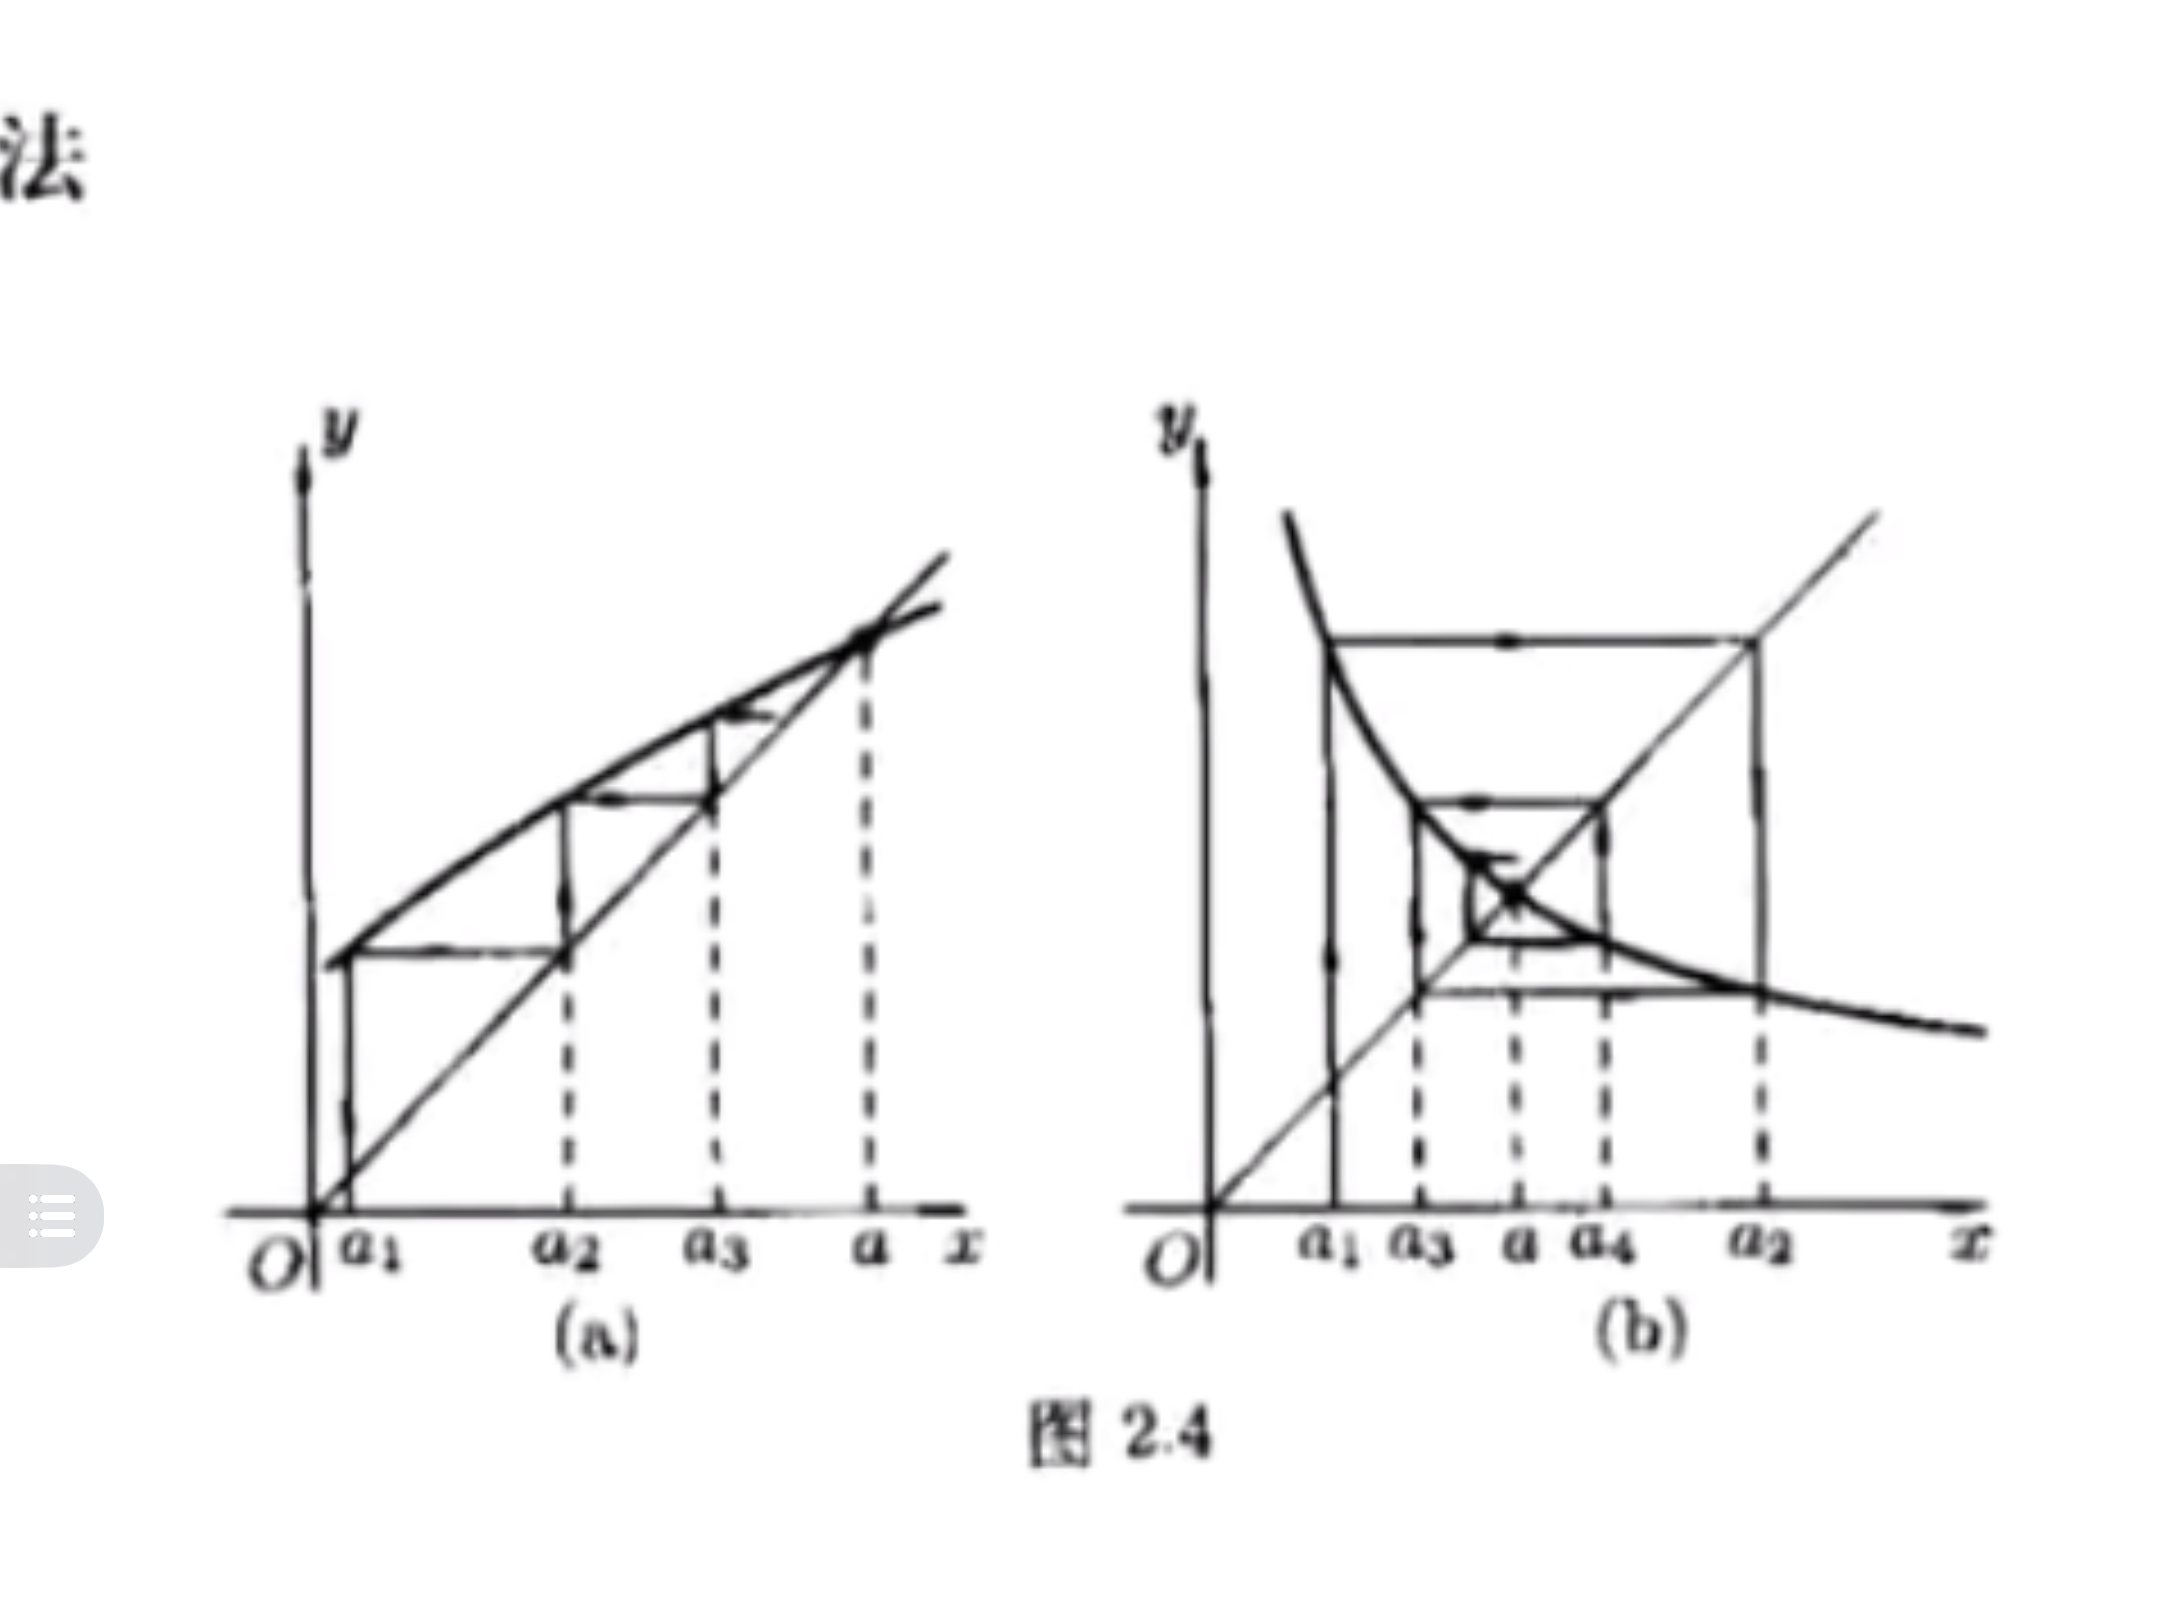
\includegraphics[width=0.5\textwidth]{figure/1.PNG}
\end{figure}
先看图2.4(a)。在其中的曲线代表函数 \( y = f(x) \)。它同直线 \( y = x \) 的交点的横坐标 \( a \) 就是 \( f \) 的不动点。从图中的 \( x \) 轴上代表初始值 \( a_1 \) 的点出发作平行于 \( y \) 轴的直线,它与曲线 \( y = f(x) \) 的交点的纵坐标就是 \( a_2 = f(a_1) \)。在这里的一个技巧是从上述交点作平行于 \( x \) 轴的直线与直线 \( y = x \) 相交。这个交点的横坐标当然也是 \( a_2 \)。在图中从这个交点作一条虚线与纵轴平行,并将它与 \( x \) 轴的交点标为 \( a_2 \)。这就完成了蛛网工作法的第一步。

在图2.4(a)上将这个方法继续做几步:可以看出,所得的数列是单调增加的

\begin{example}
	设 \( u_1 = b \), \( u_{n+1} = u_n^2 + (1 - 2a)u_n + a^2 \),试判断 \( u_n \) 的敛散性。
\end{example}

\begin{example}
	设 \( x_{n+1}(2 - x_n) = 1 \), \( n = 1, 2, \cdots \)。试判断 \( x_n \) 的敛散性。
\end{example}

\begin{example}
	定义数列 \( a_0 = x \), \( a_{n+1} = \frac{a_n^2 + y^2}{2} \), \( n = 0, 1, 2, \cdots \),记 \( D = \{(x, y) \in \mathbb{R}^2 : \text{数列 } a_n \text{ 收敛}\} \)。
\end{example}
\chapter{函数}
\section{连续性和可微性}
\subsection{定义法}
\begin{example}
	(2023 复旦应统夏令营) 若 \( f'(x_0) \) 存在,试求 \(\lim_{h \to 0} \frac{f(x_0 + ah) - f(x_0 - bh)}{h}\);反之,若 \(\lim_{h \to 0} \frac{f(x_0 + h) - f(x_0) - h}{h}\) 存在,试问 \( f(x) \) 在 \( x_0 \) 处是否可导?
\end{example}
\begin{example}
	(2021 中科院考研) 若 \( f(x) \) 在 \( x = 0 \) 处连续,且 \(\lim_{x \to 0} \frac{f(2x) - f(x)}{x} = 0\),求证:\( f'(0) = 0 \)。
\end{example}
\begin{example}
	(2024 上交夏令营) 设函数 \( f(x) \) 在 \((-\infty, +\infty)\) 上连续,且 \(\lim_{x \to 0} \frac{f(x)}{x}\) 存在,令  
\[g(x) = \int_0^1 f(xt) \, dt,\]

(1) 求 \( g'(x) \);  

(2) 讨论 \( g'(x) \) 在 \( x=0 \) 处的连续性。
\end{example}
\subsection{级数法}
\begin{example}
	(2024 同济夏令营) 设 \(\{x_n\} \subset (0,1)\), \(x_j \neq x_i\) (\(i \neq j\)), 定义函数
\[ f(x) = \sum_{n=1}^{\infty} \frac{\operatorname{sgn}(x - x_n)}{2^n}, \]
试判断 \(f(x)\) 的连续性并给出证明。

\end{example}
\begin{example}
	(2023 复旦数科院夏令营) 设数列 \(\{r_n\}\) 为 \([0,1]\) 中的所有有理点的一个排列,证明函数
\[ f(x) = \sum_{n=1}^{\infty} \frac{|x - r_n|}{3^n}, \quad x \in [0,1] \]
具有以下性质:
\begin{enumerate}
    \item[(1)] 处处连续;
    \item[(2)] 在无理点处可微,有理点处不可微。
\end{enumerate}
\end{example}
\begin{example}
	(Cantor 函数) 设 \( C \) 为 \([0,1]\) 上的 Cantor 集,对于 \( x = 2 \sum_{i=1}^{\infty} \frac{a_i}{3^i} \in C \), \( a_i \in \{0,1\} \),令  
\[ \phi(x) = \phi\left(2 \sum_{i=1}^{\infty} \frac{a_i}{3^i}\right) = \sum_{i=1}^{\infty} \frac{a_i}{2^i}. \]  
Cantor 函数 \(\phi(x)\) 定义为:\(\forall x \in [0,1]\),  
\[ \phi(x) = \sup\{\phi(y) \mid y \in C, y \leq x\}. \]  
求证:\(\phi\) 为 \([0,1]\) 上的连续函数。
\end{example}
\begin{example}
	设 \( Q = \{x_1, x_2, \cdots\} \) 为有理数集合,令  
	\[ f(x) = \sum_{x_n \leq x} \frac{1}{2^n}, \]  
	证明:\( f(x) \) 仅在有理点处不连续。
\end{example}
\subsection{Schwarz导数}
\begin{definition}
	设有定义在开集 \( A \subset \mathbb{R} \) 上的实函数 \( f(x) \),若对于 \( a \in A \),
\[ \lim_{h \to 0} \frac{f(a+h)-f(a-h)}{2h} = f^s(a) \]
存在,则称 \( f(x) \) 在点 \( a \) Schwarz 可导,称 \( f^s(a) \) 为 Schwarz 导数。

\end{definition}
\begin{proposition}
	设 \( f(x) \in C[a,b] \) 且在 \( (a,b) \) 上 Schwarz 可导,那么:
\begin{itemize}
    \item 若 \( f(b) > f(a) \),则 \( \exists\, c \in (a,b) \),使得 \( f^s(c) \geq 0 \)。
    \item 若 \( f(a) > f(b) \),则 \( \exists\, c \in (a,b) \),使得 \( f^s(c) \leq 0 \)。
\end{itemize}

\end{proposition}
\begin{theorem}[Schwarz 导数的 Rolle 中值定理]
	设 \( f(x) \in C[a, b] \) 且在 \( (a, b) \) 上 Schwarz 可导,若 \( f(a) = f(b) \),则  
\(\exists\, r, t \in (a, b) \),使得 \( f^s(r) \geq 0 \) 且 \( f^s(t) \leq 0 \)。

\end{theorem}
\begin{theorem}[Schwarz 导数的 Lagrange 中值定理]
	设 \( f(x) \in C[a, b] \) 且在 \( (a, b) \) 上 Schwarz 可导,则存在 \( r, t \in (a, b) \),使得
\[ f^s(r) \leq \frac{f(b) - f(a)}{b - a} \leq f^s(t). \]
\end{theorem}
\begin{theorem}[Schwarz 导数与一般导数的联系]
	设 \( f(x) \in C[a, b] \) 且在 \( (a, b) \) 上 Schwarz 可导,若 \( f^s(x) \) 在 \( (a, b) \) 上连续,则 \( f(x) \) 在 \( (a, b) \) 上可导且
\[ f'(x) = f^s(x), \quad \forall x \in (a, b). \]

\end{theorem}
\begin{theorem}[利用 Schwarz 导数判断函数单调性]
	设函数 \( f(x) \) 在开区间 \( I \) 上连续且 Schwarz 可导,若 \( f^s(x) \geq 0 \) 对所有 \( x \in I \) 成立,则 \( f(x) \) 在 \( I \) 上单调递增。
\end{theorem}
\section{一致连续性}
\begin{example}
	设 \( f(x) \) 在 \([a, +\infty)\) 上一致连续,\( g(x) \) 在 \([a, +\infty)\) 上连续,且
\[ \lim_{x \to +\infty} |f(x) - g(x)| = 0. \]
求证:\( g(x) \) 在 \([a, +\infty)\) 上一致连续。
\end{example}
\begin{example}
	设 \( f(x) \) 在 \([1, +\infty)\) 上一致连续。求证:存在 \( M > 0 \),使得
\[ \frac{|f(x)|}{x} \leq M, \quad \forall x \in [1, +\infty). \]
\end{example}
\begin{example}
	设 \( f(x) \) 在 \([0, +\infty)\) 上一致连续,且对任意 \( x \geq 0 \) 有
\[ \lim_{n \to +\infty} f(x+n) = 0, \quad n \in \mathbb{N}. \]
求证:
\[ \lim_{x \to +\infty} f(x) = 0. \]
\end{example}
\begin{example}
	设 \( f(x) \) 在 \([0, +\infty)\) 上连续,且满足
\[ \lim_{n \to \infty} f(\sqrt{n}) = 0. \]
求证:\(\lim_{x \to +\infty} f(x)\) 存在当且仅当 \( f(x) \) 在 \([0, +\infty)\) 上一致连续。

\end{example}
\begin{example}
	若 \( f(x) \) 在 \([0,+\infty)\) 上可导,且满足:
\begin{enumerate}
    \item \( f'(x) \) 在 \([0,+\infty)\) 上一致连续;
    \item \( \lim_{x \to +\infty} f(x) \) 存在。
\end{enumerate}
求证:
\[ \lim_{x \to +\infty} f'(x) = 0. \]
\end{example}
\begin{example}
	(2024 国防科大考研) 设函数 \( f(x) \) 在 \( (0,1] \) 上连续且可导,且满足
    \[ \lim_{x \to 0^+} \sqrt{x}f'(x) = a. \]
    求证:\( f(x) \) 在 \( (0,1] \) 上一致连续。
\end{example}
\begin{example}
	(2024 哈工大考研) 设 \( (a,b) \) 为有界开区间,求证:\( f(x) \) 在 \( (a,b) \) 上一致连续的充要条件是对于任意 Cauchy 列 \( \{x_n\} \subset (a,b) \),像列 \( \{f(x_n)\} \) 也是 Cauchy 列。
\end{example}
\begin{example}
	(2023 吉大夏令营) 设 \( f(x) \in C[1,+\infty) \),且满足
    \[ \lim_{x \to +\infty} \frac{f(x)}{x^2} = 1. \]
    求证:\( f(x) \) 在 \( [1,+\infty) \) 上非一致连续。
\end{example}
\section{函数方程}
\subsection{柯西方程}
\begin{definition}
	我们称函数 \( f \colon \mathbb{R} \to \mathbb{R} \) 满足的函数方程
\[ f(x + y) = f(x) + f(y) \]
为 \textbf{Cauchy 方程}。
\end{definition}
\begin{example}
	设 \( f \colon \mathbb{R} \to \mathbb{R} \) 是 Cauchy 方程的解,则:
\begin{enumerate}
    \item[(1)] 对任意有理数 \( r \in \mathbb{Q} \),有
    \[ f(rx) = r f(x); \]
    \item[(2)] 进一步,若 \( f \) 连续,则存在常数 \( c = f(1) \) 使得
    \[ f(x) = c x, \quad \forall x \in \mathbb{R}. \]
\end{enumerate}
\end{example}
\begin{example}
	求证:\(\mathbb{R}\) 上既凸又凹的连续函数必为线性函数,即存在常数 \( a, b \in \mathbb{R} \) 使得
\[ f(x) = a x + b, \quad \forall x \in \mathbb{R}. \]
\end{example}
\begin{example}
	设 \( f(x) \) 在 \( (0, +\infty) \) 上连续,且满足函数方程:
\[ f(xy) = x f(y) + y f(x), \quad \forall x, y \in (0, +\infty). \]
求证:\( f(x) \) 在 \( (0, +\infty) \) 上可微。
\end{example}
\begin{example}
	(2024 中科院夏令营) 证明:在 \( \mathbb{R} \) 上满足函数方程
\[ f(x+y) = f(x) f(y) \]
的唯一不恒等于零的连续解是指数函数 \( f(x) = a^x \),其中 \( a > 0 \) 为常数。
\end{example}
\subsection{迭代法}
\textbf{基本思想}:通过构造递推关系,将函数方程转化为可求和的形式。
\begin{example}
	求函数方程 
\[ 2f(2x) = f(x) + x \]
在 $\mathbb{R}$ 上且满足 $f$ 在 $x=0$ 处连续的所有解。
\end{example}
\begin{example}
	求函数方程
\[ f(x+y) - f(x-y) = f(x)f(y) \]
在 $\mathbb{R}$ 上且满足 $f$ 在 $x=0$ 处连续的所有解。
\end{example}
\begin{example}
	求函数方程 
    \[ f(\log_2 x) = f(\log_3 x) + \log_5 x \]
    在 \( \mathbb{R}^+ \) 上的所有连续解。
\end{example}

\chapter{一元函数微分学}
\section{微分中值定理}
\subsection{插值法}
有一类中值定理习题中往往会给我们很多关于函数 $f(x)$ 的信息,进而去证明一个等式。如何利用好这些已知信息?这就涉及到数值分析中的 Lagrange 插值与 Newton 插值。
\begin{theorem}[Lagrange 插值]
	已知插值节点为 $(x_i, y_i), i = 0, 1, 2, \cdots, n$,那么

\[ y = f(x) = \sum_{0 \leq i < n} \frac{(x - x_0) \cdots (x - x_{i-1})(x - x_{i+1}) \cdots (x - x_n)}{(x_i - x_0) \cdots (x_i - x_{i-1})(x_i - x_{i+1}) \cdots (x_i - x_n)} y_i \]

对应的插值余项为:

\[ R_n(x) = f(x) - L_n(x) = \frac{f^{(n+1)}(\xi)}{(n+1)!}(x - x_0)(x - x_1) \cdots (x - x_n) \]

\end{theorem}
\begin{theorem}[Newton 插值]
	已知插值节点为 $(x_i, y_i), i = 0, 1, 2, \cdots, n$,那么

\[ f(x) = a_0 + a_1(x - x_0) + a_2(x - x_0)(x - x_1) + \cdots + a_n(x - x_0)(x - x_1)(x - x_2) \cdots (x - x_{n-1}), \]

其中 $a_n = f[x_0, x_1, \cdots, x_k]$,对应的插值余项为:

\[ R_n(x) = f(x) - L_n(x) = \frac{f^{(n+1)}(\xi)}{(n+1)!}(x - x_0)(x - x_1) \cdots (x - x_n) \]

\textbf{Tip:} Newton 插值可以带重节点,进而反映出导数信息。
\end{theorem}
\begin{example}
	设 $f \in D^3[-1, 1]$,$f(-1) = 0$,$f'(0) = 0$,$f(1) = 1$。求证:$\exists \theta \in (-1, 1)$,s.t. $f'''(\theta) = 3$。
\end{example}
\begin{example}
	设 \(f \in C[0, 2] \cap D(0, 2)\) 满足 \(f(0) = f(2) = 0\), \(|f'(x)| \leq M\), \(\forall x \in (0, 2)\)。求证:
\[ \left| \int_{0}^{2} f(x) \, dx \right| \leq M. \]
\end{example}
\begin{example}
	设 \( f \in C^3[0,2] \) 满足
\[ f(0) = f'(0) = 0, \quad \int_{0}^{2} f(x) \, dx = 8 \int_{0}^{1} f(x) \, dx. \]
证明:存在 \( \theta \in (0,2) \),使得 \( f''(\theta) = 0 \)。
\end{example}
下面我们来介绍插值法的积分型余项,这种余项往往蕴含着更多的信息。
\begin{theorem}[积分型余项]
	设 \( f(x) \) 是 \([a,b]\) 上的二阶可导函数且 \( f''(x) \in R[a,b] \),则有:
\[ f(x) = \frac{b-x}{b-a}f(a) + \frac{x-a}{b-a}f(b) + \int_a^b f''(y)k(x,y)dy, \]
其中,
\[ k(x,y) = 
\begin{cases} 
\frac{(x-a)(y-b)}{b-a}, & a \leq y \leq x \leq b; \\ 
\frac{(b-x)(a-y)}{b-a}, & a \leq x \leq y \leq b.
\end{cases} \]
\end{theorem}
\begin{example}
	(2021华东师范考研压轴) 设 \( f \in C^2[0,1] \) 满足 \( f(0) = f(1) = 0 \),证明:
\[ \int_0^1 \left| \frac{f''(x)}{f(x)} \right| dx \leq 4. \]
\end{example}
\begin{example}
	设 \( f(x) \in D^2[0, 1] \), \( f(0) = f(1) = 0 \), \( |f''(x)| \leq M \), 求证:
    \[ \int_{0}^{1} f(x) \, dx \leq \frac{M}{12} \]
    
\end{example}
\begin{example}
	已知 \( f(x) \in C^2[a, b] \), \( f(a) = f(b) = 0 \), 求证:
    \[ |f(x)| \leq \frac{(x - a)(b - x)}{b - a} \int_{a}^{b} |f''(y)| \, dy \]
\end{example}
\subsection{K值法}
看例题操作,有手就行
\begin{example}
	(2021 天津大学考研) 设函数 \( f(x) \in C[a,b] \cap D^2(a,b) \),求证:\(\exists \xi \in (a,b)\),使得
\[ f(b) - 2f\left(\frac{a+b}{2}\right) + f(a) = \frac{(b-a)^2}{4}f''(\xi). \]
\end{example}
\begin{example}
	(2024 大连理工考研) 设函数 \( f(x) \) 在 \([0,2]\) 上有二阶连续导数,且 \( f(0) = f(1) = f(2) = 0 \),求证:\(\forall x \in (0,2)\),\(\exists c \in (0,2)\),使得
\[ f(x) = \frac{1}{6}x(x-1)(x-2)f'''(c). \]
\end{example}
\begin{example}
	设 $f$ 在 $[a,b]$ 上二阶可微,$f(a) = f(b) = 0$。证明:对每个 $x \in (a,b)$,存在 $\xi \in (a,b)$,使得
    \[ f(x) = \frac{f''(\xi)}{2}(x-a)(x-b). \]
\end{example}
\begin{example}
	设 $f \in D^3[0,1]$ 满足 $f(0) = -1$, $f'(0) = 0$, $f(1) = 0$。证明对任何 $x \in [0,1]$,存在 $\theta \in (0,1)$,使得
    \[ f(x) = -1 + x^2 + \frac{x^2(x-1)}{6}f'''(\theta). \]
\end{example}
\subsection{微分方程法}
有一类中值定理习题的解决需要我们构造合适的函数,我们可以通过解微分方程来得到。下面我们结合具体的例子来说明。
\begin{example}
	设函数 \( f(x) \in C[0,2] \cap D(0,2) \),且 \( f(0) = f(2) = 0 \),\(\lim\limits_{x \to 1} \frac{f(x) - 2}{x - 1} = 5\)。求证:
\[ \exists \xi \in (0,2), \text{ s.t. } f'(\xi) = \frac{2\xi - f(\xi)}{\xi}. \]
\end{example}
\begin{example}
	(2024 复旦夏令营) 设函数 \( f(x) \in C[0,1] \cap D(0,1) \),且 \( f'(1) = 0 \)。求证:
\[ \exists \xi \in (0,1), \text{ s.t. } f'(\xi) = 2024(f(\xi) - f(0)). \]
\end{example}
\begin{example}
	(2024 上海夏令营) 设 \( f(x) \) 在 \([a,b]\) 上可导,且 \(\exists c \in [a,b]\), s.t. \( f'(c) = 0 \). 求证:
\[ \exists \xi \in [a,b], \text{ s.t. } f'(\xi) = \frac{f(\xi) - f(a)}{b - a}. \]
\end{example}
\begin{example}
	设函数 \( f(x) \in C[0,1] \cap D(0,1) \),且 \( f(0) = 0 \)。求证:
    \[ \exists u \in (0,1), \text{ s.t. } f'(u) = \frac{u f(u)}{1 - u}. \]
\end{example}
\begin{example}
	设函数 \( f(x) \in C[-1,2] \cap D(-1,2) \), \( f(-1) = f(2) = -\frac{1}{2} \), \( f\left(\frac{1}{2}\right) = 1 \)。求证:
    \[ \forall \lambda \in \mathbb{R}, \exists \xi \in (-1,2), \text{ s.t. } f'(\xi) = \lambda \left|f(\xi) - \frac{\xi}{2}\right| + \frac{1}{2}. \]
\end{example}
\begin{example}
	设函数 \( f(x) \in D^2\left[0,\frac{\pi}{4}\right] \), \( f(0) = 0 \), \( f'(0) = 1 \), \( f\left(\frac{\pi}{4}\right) = 1 \)。求证:
    \[ \exists \xi \in \left(0,\frac{\pi}{4}\right), \text{ s.t. } f''(\xi) = 2f(\xi)f'(\xi). \]
\end{example}
\section{函数性态分析}
\subsection{常用结论}
\begin{theorem}
	导数大于0则函数的趋于无穷设 $f$ 在 $[0,+\infty)$ 上可微且 $\lim_{x \to +\infty} f(x) = x > 0$。求证:$\lim_{x \to +\infty} f(x) = +\infty$。
\end{theorem}
\begin{theorem}
	函数值在 $[0,+\infty)$ 处必然有趋于0的子列,设 $k \in \mathbb{N}, a \in \mathbb{R}$ 且 $f \in D^k[a,-\infty]$。若 $\lim_{x \to +\infty} |f|(x) \neq +\infty$,那么存在趋于正无穷的数列 $\{x_n\}_{n=1}^\infty \subset [0,+\infty), \forall \lim_{x \to +\infty} f^{(k)}(x_n) = 0$。
\end{theorem}
\begin{theorem}[导数极限定理]
	设 $f(x) \in C^{m,n} \cup D^m[a,b]$,且 $\lim_{x \to a_+} f'(x) = c$,存在。求证:$f(x)$ 在 $[0,+\infty)$ 处可导且 $f_+'(a) = c$。
\end{theorem}
\begin{theorem}[低阶导数控制高阶导数]
	设 $f(x)$ 在 $[0,+\infty)$ 上 $n$ 阶可微,且存在有限极限 $\lim_{x \to +\infty} f(x)$ 和 $\lim_{x \to +\infty} f^{(k)}(x)$。求证:$\forall k = 1,2,\cdots,m$,有:$\lim_{x \to +\infty} f^{(k)}(x) = 0$。
\end{theorem}
\begin{theorem}[低阶导数控制高阶导数]
	设 $f(x)$ 在 $[0,+\infty)$ 上二阶可微,且$
	|f(x)|,|f'(x)|$的上确界 $A,B$。求证:$|f(x)| \leq \sqrt{2AB}$。
\end{theorem}
\begin{theorem}[低阶导数控制高阶导数]
	设 $f(x)$ 在 $[0,+\infty)$ 上二阶可微,$\lim_{x \to \infty} f(x)=0 $,且$\lambda\in\mathbb{R} s.t.f''(x)+\lambda f'(x)$有上界,求证$\lim_{x \to \infty} f'(x)=0 $
\end{theorem}
\subsection{综合运用}
\begin{example}
	设 \( f(x) \in C(\mathbb{R}) \), \( g(x) = f(x)\int_{0}^{x} f(t) dt \) 单调递减, 求证: \( f(x) \equiv 0 \).
\end{example}
\begin{example}
	设函数 \( f(x) \) 在 \((0, +\infty)\) 上可微, 极限 \(\lim_{x \to +\infty} f(x)\) 和 \(\lim_{x \to +\infty} f'(x)\) 均存在, 求证: \(\lim_{x \to +\infty} f'(x) = 0\).
\end{example}
\begin{example}
	若 \( f'(x) \in C^2[0,1] \),\( f'(0) = 0 \),\( |f''(x)| \leq |f(x) - f(0)| \)。求证:\( f(x) \) 在 \([0,1]\) 上为常值函数。
\end{example}
\begin{example}
	设 \( f(x) \in C^2[0,1] \),\( f(0) = f(1) \),且 \( |f''(x)| \leq 2 \),\(\forall x \in [0,1]\)。  
证明:\(\forall x \in [0,1],|f'(x)| \leq 1\)。
\end{example}
\begin{example}
	设 \( f(x) \in C[0,1] \cap D(0,1) \), \( f(0) = f(1) \), 且 \( |f'(x)| < 1 \).  
求证:\( \forall x_1, x_2 \in [0,1] \), \( |f(x_1) - f(x_2)| < \frac{1}{2} \).
\end{example}
\section{函数逼近问题}
\subsection{连续函数的逼近}
\begin{theorem}[Weierstrass 第一逼近定理]
	对于闭区间 $[a, b]$ 上的任意连续函数 $f(x)$,存在多项式序列 $\{P_n\}$ 在 $[a, b]$ 上一致收敛于 $f(x)$。
\end{theorem}
\begin{theorem}[Weierstrass 第二逼近定理]
	$\mathbb{R}$上周期为 $2\pi$ 的连续函数可被三角多项式一致逼近。
\end{theorem}


\begin{example}
	设 $f(x) \in C[0, 1]$,$\forall n \in \mathbb{N}$,$\int_0^1 f(x) x^n dx = 0$,$\forall n = 0, 1, 2, \cdots$,求证:$f(x) \equiv 0, \forall x \in [0, 1]$。
\end{example}
\begin{example}[Riemann 引理]
	设函数 $f(x)$ 在 $[a, b]$ 上可积,那么有:
\[
\lim_{\lambda \to \infty} \int_a^b f(x) \sin \lambda x dx = 0, \quad \lim_{\lambda \to \infty} \int_a^b f(x) \cos \lambda x dx = 0.
\]
\end{example}
\begin{example}
	设 $f(x) \in R[a, b], g(x)$ 以 $T$ 为周期且在 $[0, T]$ 上可积,则有:
    \[
    \lim_{n \to \infty} \int_a^b f(x) g(nx) dx = \frac{1}{T} \int_0^T g(x) dx \int_a^b f(x) dx.
    \]
\end{example}
\begin{example}
	设 $f(x) \in R[a, b]$,求证:$\lim_{n \to \infty} \int_a^b f(x) \sin nx dx = \frac{2}{\pi} \int_a^b f(x) dx$。
\end{example}
\subsection{可积函数的逼近}
\begin{example}[阶梯逼近]
	设 \( f(x) \in R[a,b] \), \(\forall \epsilon > 0\), 存在 \([a,b]\) 上的阶梯函数 \( g(x) \), 使得 
\[ \int_{a}^{b} |f(x)-g(x)|dx \leq \epsilon. \]
\end{example}
\begin{example}[连续逼近]
	设 \( f(x) \in R[a,b] \), \(\forall \epsilon > 0\), 存在 \( g(x) \in C[a,b] \), 使得 
\[ \int_{a}^{b} |f(x)-g(x)|dx < \epsilon. \]
\end{example}
\begin{example}[可微逼近]
	设 \( f(x) \in R[a,b] \), \(\forall \epsilon > 0\), 存在 \( g(x) \in C^{1}[a,b] \), 使得 
\[ \int_{a}^{b} |f(x)-g(x)|dx < \epsilon. \]
\end{example}
\begin{example}[绝对连续性]
	设 \( f(x) \) 在任意有限区间可积,证明:\(\forall [a,b]\), 有:
\[ \lim_{h \to 0} \int_{a}^{b} |f(x+h)-f(x)|dx = 0. \]
\end{example}
\begin{example}
	设 \( f(x) \in R[a,b] \), \( F(x) = \int_{a}^{x} f(t)dt \). 求证:
\[ \int_{a}^{b} F(x)dx = \int_{a}^{b} (b-x)f(x)dx. \]
\end{example}

\chapter{一元函数积分学}
\section{积分的计算}
\subsection{区间再现公式}
\begin{example}[区间再现公式]
	求 \( \int_{a}^{b} f(x) dx - \int_{a}^{b} f(a+b-x) dx = \frac{1}{2} \int_{a}^{b} [f(x)+f(a+b-x)] dx \)。
	\end{example}
	
	\begin{example}
	计算:
	\[(1) \int_{0}^{1} \ln a \ln x dx, \quad (2) \int_{0}^{1} \frac{\ln(1+x)}{1+x^2} dx.\]
	\end{example}
	
\begin{example}
	计算:
	\[(1) \int_{0}^{\infty} \frac{dx}{(1+x^2)(1+x^a)} \ (a>0), \quad (2) \int_{0}^{\infty} \frac{\ln x}{x^2 + x + 1 }dx.\]
\end{example}
\begin{example}
	计算
	\[\int_{0}^{\frac{\pi}{2}}\frac{e^{\sin x}}{e^{\sin x}+e^{\cos x}}  \,dx 
	\]
\end{example}
\begin{example}
	对$n\in\mathbb{N} $计算
	\[\int_{0}^{2\pi}  \sin(\sin x+nx )\,dx 
	\]
\end{example}
\subsection{Froullani积分}
\begin{example}[Froullani积分]
	设 \( f \in C(0,+\infty) \),若存在极限  
	\[\lim_{x \to 0^+} f(x), \quad \lim_{x \to +\infty} f(x)\]  
	则有:  
	\[\int_0^\infty \frac{f(ax) - f(bx)}{x} dx = \left[ \lim_{x \to 0^+} f(x) - \lim_{x \to +\infty} f(x) \right] \ln \frac{b}{a}\]
\end{example}
	
\begin{example}
	计算  
	\[\int_0^{+\infty} \left( \frac{\sin 3x}{3x^2} - \frac{\sin 2x}{2x^2} \right) dx\]
\end{example}
	
\begin{example}
	计算 \[ \int_{0}^{\infty} \frac{\cos ax - \cos bx}{x} dx, \quad b > a > 0. \]
\end{example}
\begin{example}
	\begin{enumerate}
		\item 若存在极限和积分 \[ \lim_{x \to 0} f(x) = 0, \quad \int_{a}^{b} \frac{f(x)}{x} dx \],求证:
		\[ \forall a, b > 0, \int_{0}^{a} \frac{f(ax) - f(bx)}{x} dx = a \ln \frac{b}{a};\]
		\item 若存在极限和积分 \[ \lim_{x \to \infty} f(x) = 0, \quad \int_{0}^{a} \frac{f(x)}{x} dx \],求证:
		\[ \forall a, b > 0, \int_{0}^{a} \frac{f(ax) - f(bx)}{x} dx = a \ln \frac{b}{a}.\]
	\end{enumerate}
\end{example}
\subsection{化为含参积分处理}
\begin{example}
	计算 \[ \int_{0}^{1} \frac{\arctan x}{x\sqrt{1-x^2}} \, dx \]
	\end{example}
	
	\begin{example}
	计算 \( I(y) = \int_{0}^{\infty} e^{-x^2} \cos 2xy \, dx, \quad y \in \mathbb{R} \).
	\end{example}
	
	\begin{example}
	计算 \( \int_{0}^{\infty} \frac{\arctan ax}{x(1+x^2)} \, dx \).
	\end{example}
\begin{example}
	计算
	\[\int_{0}^{+\infty}\frac{\cos x-\cos 2x}{x}e^{-x}  \,dx 
	\]
\end{example}
\begin{example}
	计算
	\[\int_{0}^{+\infty}\frac{\sin bx-\sin ax}{x}e^{-px}  \,dx ,p>0,b>a
	\]
\end{example}

\subsection{级数方法}
为了换序 \(\sum_{n=1}^{\infty} \int_{a}^{b} f_n(x) dx = \int_{a}^{b} \sum_{n=1}^{\infty} f_n(x) dx\),我们需要:

\[\lim_{m \to \infty} \sum_{n=1}^{m} \int_{a}^{b} f_n(x) dx = \int_{a}^{b} \sum_{n=1}^{\infty} f_n(x) dx.\]

有限和随意交换,我们需要:

\[\lim_{m \to \infty} \int_{a}^{b} \sum_{n=1}^{m} f_n(x) dx = \int_{a}^{b} \sum_{n=1}^{\infty} f_n(x) dx.\]

于是需要:

\[\lim_{m \to \infty} \int_{a}^{b} \sum_{n=m+1}^{\infty} f_n(x) dx = 0.\]

\begin{example}
计算:\(\int_{0}^{\infty} \frac{x}{1+e^x} dx\).
\end{example}

\begin{example}
计算:\(\int_{0}^{\infty} \frac{\ln x}{1-x^2} dx\).
\end{example}

\begin{example}
计算:  
\[\int_{0}^{1} \ln x \ln (1 - x) dx \]
\end{example}
\begin{example}
	计算积分:\[\int_{0}^{1} \frac{\ln (1 + x + x^2)}{x} dx.\]
\end{example}
\begin{example}
	计算积分:\[\int_{0}^{+\infty} \frac{x - [x] - \frac{1}{2}}{x} dx.\]
\end{example}
\section{积分的渐进展开}
\subsection{定积分定义}
\begin{example}
	设 \( f \) 在 \([0,1]\) 上可微,\(\left|f'(x)\right| < M\),证明:
\[
\left|\int_0^1 f(x) \, dx - \frac{1}{n} \sum_{k=1}^n f\left(\frac{k}{n}\right)\right| \leq \frac{M}{2n}.\]
\end{example}
\begin{example}
	设 \( f(x) \) 在 \([0,1]\) 可微且导数在 \([0,1]\) 上黎曼可积,则有:
\[
\lim_{n \to \infty} n \left( \frac{1}{n} \sum_{k=1}^n f\left(\frac{k}{n}\right) - \int_0^1 f(x) \, dx \right) = \frac{f(1) - f(0)}{2}.
\]
\end{example}
\begin{example}
	设 \( f \) 在区间 \([0,1]\) 上二阶可微,且 \( f'' \in R[0,1] \),求证:
\[
\lim_{n \to \infty} n^2 \left( \int_0^1 f(x) \, dx - \frac{1}{n} \sum_{k=1}^n f\left(\frac{2k-1}{2n}\right) \right) = \frac{1}{24} [f'(1) - f'(0)].
\]
\end{example}
\begin{example}
	设 \( f(x) \) 在 \([0,1]\) 上 \(2m\) 阶可微且 \(2m\) 阶导数在 \([0,1]\) 上勒贝格可积,则有:
\[
\frac{1}{n} \sum_{k=1}^n f\left(\frac{k}{n}\right) = \frac{f(1) - f(0)}{2n} + \int_0^1 f(x) \, dx + \sum_{k=1}^m \frac{\left(f^{(2k-1)}(1) - f^{(2k-1)}(0)\right)}{n^{2k}} b_{2k}(0) + o\left(\frac{1}{n^{2m}}\right).
\]
\end{example}
\begin{example}
	设 \( f(x) = \arctan x \),\( A \) 为常数,若
	\[
	B = \lim_{n \to \infty} \left( \sum_{k=1}^n f\left(\frac{k}{n}\right) - A n \right)
	\]
	存在,求 \( A \) 和 \( B \)。
\end{example}
\subsection{Euler-Maclaurin公式}
\begin{theorem}[0 阶情形]
	设 \( a, b \in \mathbb{Z} \),\( f(x) \in D^1[a, b] \),\( f'(x) \in L^1[a, b] \),则有:
\[
\sum_{k=a}^b f(k) = \int_a^b f(x) \, dx + \frac{f(a) + f(b)}{2} + \int_a^b \left( [x] - \frac{1}{2} \right) f'(x) \, dx.
\]

\end{theorem}
\begin{theorem}[一般情形(了解即可,本质上是分部积分)]
	设 \( a, b, m \in \mathbb{Z} \),\( m \geq 2 \),\( f(x) \in D^m[a, b] \),\( f^{(m)}(x) \in L^1[a, b] \),则有:
	\[
	\sum_{k=a}^b f(k) = \int_a^b f(x) \, dx + \frac{f(b) + f(a)}{2} + \sum_{k=2}^m \frac{f^{(k-1)}(b) - f^{(k-1)}(a)}{k!} (b - a)^k + (-1)^{m+1} \int_a^b B_m(x) f^{(m)}(x) \, dx.
	\]
\end{theorem}
\begin{example}
	设 \( f \in C^2[0, h] \),则存在 \( \xi \in [0, h] \),使得:
\[
\int_0^h f(x) \, dx = \frac{h}{2} [f(0) + f(h)] - \frac{1}{12} f''(\xi) h^3.
\]
\end{example}
\begin{example}
	设 \( f \in C^4[0, h] \),则存在 \( \xi \in [0, h] \),使得:
\[
\int_0^h f(x) \, dx = \frac{h}{2} [f(0) + f(h)] - \frac{h^2}{12} [f'(h) - f'(0)] + \frac{1}{720} f^{(4)}(\xi) h^5.
\]
\end{example}
\textbf{利用 Euler-Maclaurin 公式,我们可以导出很多渐近展开:}
\begin{itemize}
    \item \(\sum_{k=1}^n \frac{1}{k} \sim \ln n + \frac{1}{2n} - \frac{1}{12n^2} + \frac{1}{120n^4} + \cdots\)
    \item \(\ln(n!) \approx n \ln n - n + \frac{1}{2} \ln(2\pi n) + \frac{1}{12n} - \frac{1}{360n^3} + \cdots\)
\end{itemize}
\section{积分不等式}
\subsection{Cauchy不等式}
\begin{example}[Cauchy不等式]
	设 \( f(x), g(x) \in R[a, b] \),则有:
\[
\left( \int_a^b f(x) g(x) \, dx \right)^2 \leq \left( \int_a^b f^2(x) \, dx \right) \left( \int_a^b g^2(x) \, dx \right).
\]
\end{example}
\begin{example}
	(第十一届全国大学生数学竞赛) 设 \( f(x) \in C[0,1] \),且 \( 1 \leq f(x) \leq 3 \),求证:
\[
1 \leq \int_0^1 f(x) \, dx \int_0^1 \frac{1}{f(x)} \, dx \leq \frac{4}{3}.
\]
\end{example}
\begin{example}
	设 \( f(x) \in C^1[a, b] \),\( f(a) = 0 \),求证:
\[
\int_a^b f^2(x) \, dx \leq \frac{(b - a)^2}{2} \int_a^b f'^2(x) \, dx.
\]
\end{example}
\begin{example}
	设 \( f(x): [0,1] \to \mathbb{R} \),且 \(\int_0^1 x f(x) \, dx = 0\),求证:
\[
\int_0^1 f^2(x) \, dx \geq 4 \left( \int_0^1 f(x) \, dx \right)^2.
\]
\end{example}
\begin{example}
	(2024 厦门大学数学夏令营) 设 \( f(x) \in C[a, b] \),\( f(a) = 0 \),求证:
\[
\int_a^b f^2(x) \, dx \leq \frac{(b - a)^2}{2} \int_a^b [f'(x)]^2 \, dx - \frac{1}{2} \int_a^b [f'(x)]^2 (x - a)^2 \, dx.
\]
\end{example}
\begin{example}
	已知 \( f(x) \geq 0 \),\( f(x) \in C[a, b] \),\(\int_a^b f(x) \, dx = 1\),\( k \) 为任意实数,求证:
    \[
    \left( \int_a^b f(x) \cos kx \, dx \right)^2 + \left( \int_a^b f(x) \sin kx \, dx \right)^2 \leq 1.
    \]
\end{example}
\begin{example}
	设 \( f(x) \in C^1[a, b] \),\( f(a) = f(b) = 0 \),求证:
    \[
    \int_a^b f^2(x) \, dx \leq \frac{(b - a)^2}{4} \int_a^b f'^2(x) \, dx.
    \]
\end{example}
\begin{example}
	设 \( f(x, y) \in C[a, b] \),求证:
    \[
    \iint_{D} e^{f(x) - f(y)} \, dx \, dy \geq (a - b)^2, \quad D = [a, b] \times [a, b].
    \]
\end{example}
\subsection{Jensen不等式}
\begin{example}[Jensen不等式]
	设 \( f(x) \in R[a, b] \),且 \( m \leq f(x) \leq M \),\(\phi(x)\) 为 \([m, M]\) 上的连续下凸函数,则有:
\[
\phi\left( \frac{1}{b - a} \int_a^b f(x) \, dx \right) \leq \frac{1}{b - a} \int_a^b \phi(f(x)) \, dx.
\]
\end{example}
\begin{example}
	设 \( f(x) \in C[0,1] \),\(\forall x, y \in [0,1]\),\( f\left( \frac{x + y}{2} \right) \leq \frac{f(x) + f(y)}{2} \),求证:
\[
\int_0^1 f(x) \, dx \leq f\left( \frac{1}{2} \right).
\]
\end{example}
\begin{example}
	(2023 中科院提前批) 设函数 \( f(x) \) 在 \([a, b]\) 上二阶可导,且 \( f''(x) > 0 \),求证:
\begin{itemize}
    \item[(1)] \( f\left( \frac{a + b}{2} \right) \leq \frac{1}{b - a} \int_a^b f(x) \, dx \);
    \item[(2)] 若 \( f(x) \leq 0 \),\( x \in [a, b] \),则有:
    \[
    f(x) \geq \frac{2}{b - a} \int_a^b f(x) \, dx.
    \]
\end{itemize}
\end{example}
\begin{example}
	(Hardmard 不等式) 设 \( f(x) \in C^2[a, b] \),\( f''(x) > 0 \),求证:
\[
f\left( \frac{a + b}{2} \right) \leq \frac{1}{b - a} \int_a^b f(x) \, dx \leq \frac{f(a) + f(b)}{2}.
\]
\end{example}
\begin{example}
	求证:设 \( f(x) \in C[0,1] \),\( f(x) > 0 \),则有:
    \[
    \ln \int_0^1 f(x) \, dx \geq \int_0^1 \ln f(x) \, dx.
    \]
\end{example}
\begin{example}
	设 \( f(x) \) 是 \([0,1]\) 上非负连续的凹函数,且 \( f(0) = 1 \),求证:
    \[
    2 \int_0^1 f(x) \, dx + \frac{1}{12} \leq \left( \int_0^1 f(x) \, dx \right)^2.
    \]
\end{example}
\subsection{Chebyshev不等式}
\begin{example}[Chebyshev不等式]
	设 \( f(x), g(x) \in C[a, b] \),且 \( f(x), g(x) \) 在 \([a, b]\) 上单调性一致,求证:
\[
\int_a^b f(x) \, dx \int_a^b g(x) \, dx \leq (b - a) \int_a^b f(x) g(x) \, dx.
\]
\end{example}
\begin{remark}
	若 \( f(x), g(x) \) 单调性不一致,则上述不等式反号。
\end{remark}
\begin{example}
	求证:
\[
\int_0^{\frac{1}{2}} \frac{\sin x}{1 + x^2} \, dx \leq \int_{\frac{1}{2}}^1 \frac{\cos x}{1 + x^2} \, dx.
\]
\end{example}
\begin{example}
	证明:
\[
\int_0^1 \frac{\sin x}{1 + x^2} \, dx \leq \int_0^1 \frac{\cos x}{1 + x^2} \, dx.
\]
\end{example}
\begin{example}
	证明 Chebyshev 的一般形式,即:若 \( f(x), g(x), p(x) \in C[a, b] \),且 \(\forall x \in [a, b]\),\( p(x) \geq 0 \),\( f(x), g(x) \) 的单调性一致,则有:
\[
\int_a^b p(x) f(x) \, dx \int_a^b p(x) g(x) \, dx \leq \int_a^b p(x) \, dx \int_a^b p(x) f(x) g(x) \, dx.
\]
\end{example}
\begin{example}
	设 \( f(x) \in C[0,1] \) 且单调递增,求证:
\[
\frac{\int_0^1 x f^2(x) \, dx}{\int_0^1 x f(x) \, dx} \geq \frac{\int_0^1 f^2(x) \, dx}{\int_0^1 f(x) \, dx}.
\]
\end{example}
\subsection{Opial不等式}
\begin{example}[Opial不等式]
	设 \( f(x) \in C^1[0, a] \) 且 \( f(0) = 0 \),求证:
\[
\int_0^a |f(x) f'(x)| \, dx \leq \frac{a}{2} \int_0^a f'^2(x) \, dx.
\]
\end{example}
\begin{example}
	设 \( f(x) \in C^1[0, a] \) 且 \( f(0) = f(a) = 0 \),求证:
\[
\int_0^a |f(x) f'(x)| \, dx \leq \frac{a}{4} \int_0^a f'^2(x) \, dx.
\]
\end{example}
\subsection{Young不等式}
\begin{example}
	设 \( f(x) \in C[0, c] \) (\( c > 0 \)) 且严格递增,若 \( f(0) = 0 \) 且 \( a \in [0, c] \),\( b \in [0, f(c)] \),则:
\[
\int_0^a f(x) \, dx + \int_0^b f^{-1}(x) \, dx \geq ab.
\]
\end{example}
\subsection{单调性方法}
\begin{example}
	设 \( f(x) \in C[0,1] \) 且单调递减,求证:\(\forall a \in (0,1)\),
\[
\int_0^a f(x) \, dx \geq a \int_0^1 f(x) \, dx.
\]
\end{example}
\begin{example}
	设 \( f(x) \in C[0,1] \),且 \( 0 \leq f(x) \leq x \),求证:
\[
\int_0^1 x^2 f(x) \, dx \geq \left( \int_0^1 f(x) \, dx \right)^2.
\]
\end{example}
\subsection{中值定理}
\begin{example}
	设 \( f(x) \in C^2[0,1] \),求证:
\[
\max_{x \in [0,1]} |f'(x)| \leq |f(1) - f(0)| + \int_0^1 |f''(x)| \, dx.
\]
\end{example}
\begin{example}
	设 \( f(x) \in C^1[0,2] \),\(|f'(x)| \leq 1\),\( f(0) = f(2) = 1 \),求证:
\[
1 \leq \int_0^2 f(x) \, dx \leq 3.
\]
\end{example}











\end{document}